\section{The Models}
\label{sec:models}

The real-time nature of this application suggests that
a recursive Bayesian filtering approach would be appropriate, as is often used in
real-time tracking and robotics applications.
We are using two separate models, one each for the vehicle and network states.
In each,
we assume an underlying Markov process with state $\mathcal{X}_k$,
of which observations $\mathcal{Y}_k$ are made,
giving us to the following general model,
\begin{equation}
\label{eq:rbe_model}
\begin{split}
\mathcal{X}_k &= f(\mathcal{X}_{k-1}, \omega_k) \\
\mathcal{Y}_k &= h(\mathcal{X}_k, \nu_k)
\end{split}
\end{equation}
where $\omega_k\sim\mathrm{N}(0,\mathcal{Q})$ is the system noise,
and $\nu_k\sim\mathrm{N}(0,\mathcal{R})$ is measurement error.
The transition function $f$ determines the relationship between consecutive states,
while the measurement function $h$ is a deterministic function describing the
relationship between the underlying and observed states.

The following sections describe the two Bayesian filter models based on (\ref{eq:rbe_model}) used in this application.
The first is implemented using a particle filter to estimate vehicle states,
with the primary objective of estimating vehicle travel times along roads,
while the second using these estimated times to update road states,
and is implemented using a variant of the Kalman filter referred to as the \emph{information filter}
\citep{}.

\subsection{Real-time vehicle model}
\label{sec:pf}

The underlying vehicle state at time $t_k$ consists of
the vehicle's distance traveled $x$ in meters along the route and
its speed $\dot x$ in meters per second.
Additionally, we include travel times along road segments along the route, 
$\bz = (z_1,\ldots,z_L)^\top$, in seconds,
which are independent of time but included in the state as they are estimated
sequentially as the vehicle traverses the route.
These are combined into the state vector,
\begin{equation}
\label{eq:vehicle_state}
\bX_k = 
\begin{bmatrix}
    x_k \\ \dot x_k \\ \bz
\end{bmatrix}.
\end{equation}
Observations of the vehicle are made using a GPS at time $t_k$,
giving the longitude $\lambda_k$ and latitude $\phi_k$ of the vehicle
and stored in the observation vector
\begin{equation}
\label{eq:vehicle_obs}
\bY_k = \begin{bmatrix} \lambda_k \\ \phi_k \end{bmatrix}.
\end{equation}


We chose to employ a particle filter to estimate $\bX_k$,
to do its high flexibility and use in recent 
transit vehicle modeling applications \citep{Hans_2015}.
Our main justification for using it is that it handles multimodality very well,
as demonstrated in figure~\ref{fig:pf_state},
which is a common feature of the proposal distribution particularly around bus stops.
Another advantage is the intuitive likelihood function (see section~\ref{sec:pf_update}).
Conversely, the particle filter is a computationally demanding method,
as thousands of particles are required per bus.
Section~\ref{sec:rt} describes how we were able to implement the particle filter in real-time and the timings.


In the particle filter, the posterior distribution of the state at time $t_{k-1}$,
is represented by a set of discrete points, or particles, (fig~\ref{fig:pf_state_prev})
\begin{equation}
p(\bX_{k-1} | \bY_{k-1}) \approx \tilde\bX_{k-1|k-1} := (\bX_{k-1}^{(i)})_{i=1}^N
\end{equation}
each of which is independently updated or \emph{mutated} using the transition function $f$ (fig~\ref{fig:pf_state_predict})
\begin{equation}
p(\bX_k | \bX_{k-1}) \approx \tilde\bX_{k|k-1} := 
\left(f(\bX_{k-1}^{(i)}, \psi)\right)_{i=1}^N
\end{equation}
using a parameter vector $\psi$ containing all of the necessary parameters
for the model (including system noise).
After mutation, \emph{selection} of a new set of particles is performed by
importance resampling using likelihood weights,
determined by distance between particle's map position and $\bY_k$ 
to obtain a new sample $\tilde\bX_{k|k}$, (fig~\ref{fig:pf_state_update}).


\begin{figure}[tb]
    \centering
    \begin{subfigure}[t]{0.48\textwidth}
        \centering
        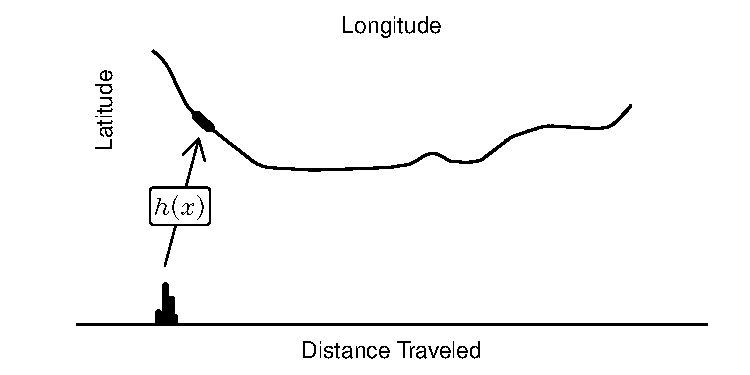
\includegraphics[width=\textwidth]{figures/03_particle_filter_1.pdf}
        \caption{The vehicle state represented by a sample of discrete points is related to the observable state (GPS position) through the transition function $h$.}
        \label{fig:pf_state_prev}
    \end{subfigure}\;\;
    \begin{subfigure}[t]{0.48\textwidth}
        \centering
        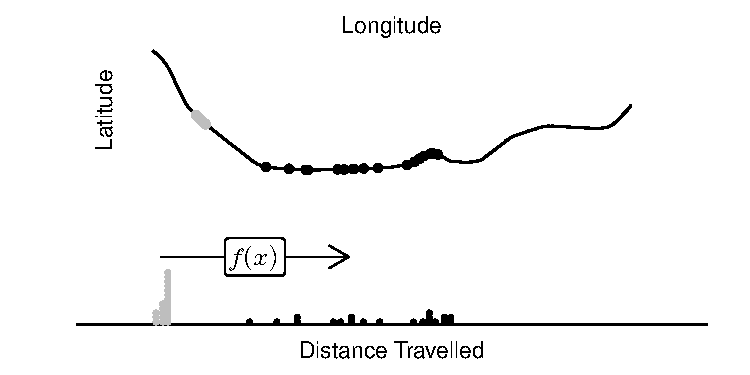
\includegraphics[width=\textwidth]{figures/03_particle_filter_2.pdf}
        \caption{The transition function $f$ models the behaviour of each particle,
            including changes in acceleration and stopping behaviour at bus stops.}
        \label{fig:pf_state_predict}
    \end{subfigure}\\
    \begin{subfigure}[t]{0.48\textwidth}
        \centering
        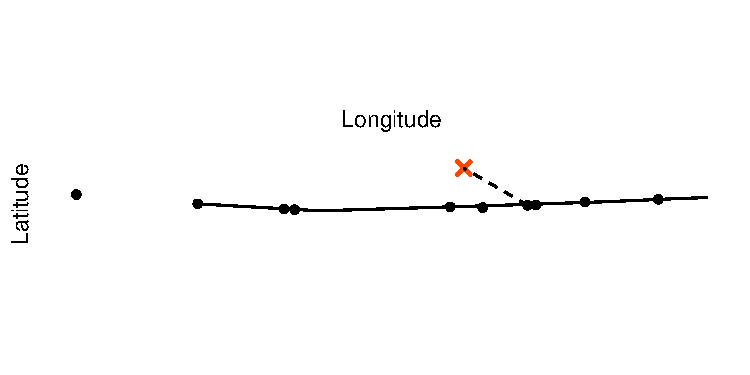
\includegraphics[width=\textwidth]{figures/03_particle_filter_6.pdf}
        \caption{Each particle's distance from the true observation is calculated using
            the geographic distance between two coordinates, which can then be used
            to calculate it's weight.}
        \label{fig:pf_state_update}
    \end{subfigure}\;\;
    \begin{subfigure}[t]{0.48\textwidth}
        \centering
        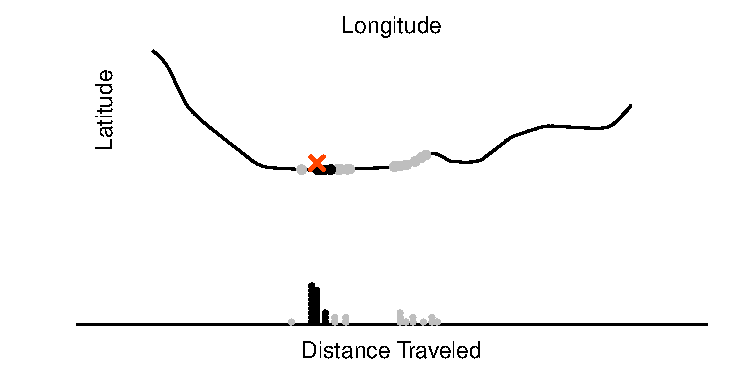
\includegraphics[width=\textwidth]{figures/03_particle_filter_4.pdf}
        \caption{Resampling occurs using likelihood weights that use the distance
            between the particle's location and the vehicles reported location (red cross),
            resulting in the updated state.}
        \label{fig:pf_state_predict2}
    \end{subfigure}
    \caption{The vehicles state is estimated using a set of discrete points, or particles,
        each of which is independently mutated to make predictions of the future state. The history of the state estimates can be used to estimate parameters of interest, such as
        travel times along roads.}
    \label{fig:pf_state}
\end{figure}



\subsubsection{Vehicle transition function}
\label{sec:pf_prediction}

Another advantage of using a particle filter to implement the vehicle model is that
the transition function $f$ can implement several bus behaviours,
most importantly
\begin{itemize}
\item non-constant speed along roads (acceleration as system noise),
\item optional stopping and waiting at bus stops while passengers board and disembark, and
\item optional stopping and waiting at intersections.
\end{itemize}

For each particle, the transition function generates a plausible trajectory,
using system noise parameter $\sigma^2$ which describes 
how the vehicles acceleration changes as a random process.
However, the vehicle does not travel constantly along the route,
as it needs to service bus stops along the way.
Therefore, the transition function includes 
stopping probabilities $\boldsymbol\pi = (\pi_1,\ldots,\pi_J)^\top$ at bus stops,
dwell times $\boldsymbol\tau = (\tau_1,\ldots,\tau_J)^\top$ for passengers to
board and disembark (conditional on the bus stopping),
and the minimum dwell time at stops, $\gamma$.
For these parameters, we used constant values for all stops,
and based the values on those used by \cite{Hans_2015};
future work will look at modeling these separately in real-time similarly to \ref{sec:kf}.
As we are using bus stops to determined segments,
no intersection model is required,
only the segment travel times as predicted by the network model at time $t_k$,
$\btheta(t_k) = (\theta_1(t_k), \ldots, \theta_L(t_k))^\top$
(see section~\ref{sec:kf}).
Future work will adapt this to use intersection that are indpendent 
of bus stops, and therefore completely independent of routes,
which will allow increasing the complexity of the model to incorporate
intersection stopping probabilities and waiting times.
The details of the transition function are given in the algorithm defined in the Appendix,
which implements those features discussed above.



\subsubsection{Updating state using the observation likelihood}
\label{sec:pf_update}

After mutating the particle set, the posterior distribution $\tilde\bX_{k|k}$ is obtained by
\emph{selection}, which is implemented by importance resampling using
likelihood weights.
To do so, we define the measurement function $h$,
and an additional function $g$ which transforms GPS coordinates onto a flat
surface (the geographical equirectangular projection),
which allows us to place a bivate normal likelihood on the data
as shown in figure~\ref{fig:pf_lhood},
The model for the observation generation is,
assuming GPS error $\epsilon^2$,
\begin{equation}
\label{eq:pf_obs_model}
g(\bY_k) = g(h(\bX_k)) + \br_k,
\quad \br_k \sim \mathrm{N}(\boldsymbol{0}, \epsilon^2\boldsymbol{I})
\end{equation}
However, due to the assumption that error in longitude and latitude are uncorrelated, 
the geographical distance between the observation and the true vehicle can be expressed
in terms of two independent standard normal random variables $z_1$ and $z_2$
\begin{equation}
\label{eq:obs_dist}
dist(\bY_k, h(\bX_k)) = \sqrt{r_{k1}^2 + r_{k2}^2} 
    = \sqrt{(\epsilon z_1)^2 + (\epsilon z_2)^2}
\end{equation}
As the sum of two independent, standard normal random variables 
is $\chi^2$ distributed with 2~degrees of freedom,
which is itself exponential,
rearranging (\ref{eq:obs_dist}) yields
\begin{equation}
\label{eq:obs_exp}
\left(\frac{dist(\bY_k, h(\bX_k))}{\epsilon}\right)^2 =
z_1^2 + z_2^2 \sim \mathrm{Exp}\left(\frac{1}{2}\right)
\end{equation}

The likelihood of the data given a particle's state estimate 
is therefore easy to calculate using (\ref{eq:obs_exp})
\begin{equation}
p(\bY_k | \bX_k^{(i)}, \epsilon) =
\frac{1}{2}\exp\left\{
-\frac{1}{2} \left(\frac{dist(\bY_k, h(\bX_k^{(i)}))}{\epsilon}\right)^2
\right\}
\end{equation}
It is worth noting that this representation of the likelihood is only
possible within the particle filter;
in other approaches, such as the Kalman filter,
the likelihood cannot be calculated using the distance as the estimate
is a distribution, and so instead a reverse non-deterministic transformation
is required, which introduces additional error and uncertainty into the model.

The posterior distribution is obtained by \emph{selection},
or resampling with replacement using the likelihood weights
\begin{equation*}
W_k^{(i)} = \frac{p(\bY_k | \bX_k^{(i)}, \epsilon)}{
    \sum_{j=1}^N p(\bY_k | \bX_k^{(j)}, \epsilon)
} 
W_{k-1}^{(i)} 
\end{equation*}
However, to improve efficiency, the state $\tilde \bX_k$ is only resampled
when the effective sample size 
$N_{\text{eff}}$ is less than some threshold,
\begin{equation*}
N_{\text{eff}} = \frac{1}{\sum_{i=1}^N (W_k^{(i)})} < N_{\text{thres}}
\end{equation*}
When resampling is performed, $W_k^{(i)} := N^{-1}$ for all $i$.
When sampling is not performed,
state estimates use $\{\bX_k^{(i)}, W_k^{(i)}\}$ to obtain weighted estimates.


\subsection{Network model}
\label{sec:kf}

[[  blurb  ]]
% The second part of this appraoch involves a network model of transit network travel times along links in the network.
% Reliable ETAs will require a historical data component,
% used as a prior in the absense of data as well as for
% predicting future states, 
% and a realtime update component where the travel times of vehicles
% are used to update the current estimate of network state.

To obtain reliable ETAs,
it is necessary to estimate travel times along roads,
as this allows the model to react to \rt congestion as detected by other buses.
Future work will aim to construct a more complex model incorporating historical trends 
and correlations between roads, 
however for the current work we are demonstrating our approach
using a simple model.

The model assums a Gaussian state distribution for travel time,
truncated necessarily at zero;
this will not be an issue as the state prediction and data will always be non-negative.
However, the model must be able to handle multiple observations in a single update,
which often occurs along major bus routes when several buses are traveling together.
Therefore we have chosen the information filter as our estimation method.

The information filter is a transormation of the Kalman filter in which the
\emph{information matrix} and \emph{information vector} are used in place of 
the covariance matrix and state vector, respectively.
The advantage is that multiple observations can be added together when updating the state.
Otherwise the information filter follows the same procedure as other recursive Bayesian models.

The network state $\boldsymbol\theta_c = \{\theta_c^\ell\}_{\ell = 1}^L$ is the travel time 
of transit vehicles along road segment $\ell$ at time $t_c$.
Observations of the state, $Z_c^\ell$, are obtained from the particle filter above.
We are assuming independence between each segment
to provide a simple basis for the model; of course in reality this
is not true and future work will investigate ways of incorporating this.
Thanks to the model simplicity,
no transition matrix or measurement matrix is required,
and the model from (\ref{eq:rbe_model}) reduces to
\begin{equation}
\begin{split}
\hat \theta_c^\ell &= \theta_{c-1}^\ell + \Delta_c^\ell v_c^\ell \\
Z_c^\ell &= \theta_c^\ell + e_c^\ell
\end{split}
\end{equation}
where $\Delta_c = t_c - t_{c-1}$,
$v_c^\ell \sim \mathrm{N}(0, \nu^2)$ is the system noise,
and $e_c^\ell \sim \mathrm{N}(0, R_c^\ell)$ is the measurement error
as estimated from the vehicle model using particle uncertainty.

The state is estimated by its mean $\hat \theta_c^\ell = \mathrm{E}(\theta_c^\ell)$
and uncertainty $P_c^\ell = \mathrm{var}(\theta_c^\ell)$,
which are predicted from the previous state estimate using the prediction
equations
\begin{align*}
\label{eq:kf_transition}
\hat \theta^\ell_{c|c-1} &= \hat \theta^\ell_{c|c-1} \\
P^\ell_{c|c-1} &= P^\ell_{c-1|c-1} + \Delta_c^\ell \nu_c^\ell
\end{align*}

For the update step, the parameters are transformed into an information
space parameterised by the information matrix $U^\ell_c$
and the information vector $u^\ell_c$,
\begin{equation}
\label{eq:information_transform}
U^\ell_{c|c-1} = \frac{1}{P_{c|c-1}}
\quad\text{and}\quad
\hat u^\ell_{c|c-1} = \frac{\hat \theta^\ell_{c|c-1}}{P^\ell_{c|c-1}}
\end{equation}
The measurement data obtained from the vehicle model are
the travel time of vehicle $m$ along segment $\ell$,
$\bar z_c^{m\ell}$, and the uncertainty $s^{m\ell}_c$.
These are transformed to a measurement information covariance matrix $B$
and vector $b$ using
\begin{equation*}
B^{m\ell}_c = \frac{1}{(s^{m\ell}_c)^{2}}\quad\text{and}\quad
b^{m\ell}_c = \frac{\bar z^{m\ell}_c}{(s^{m\ell}_c)^2}
\end{equation*}
The information update is now the sum of the information for all vehicles
that traversed the segment since the last update, so
\begin{align*}
U^\ell_{c|c} &= U^\ell_{c|c-1} + \sum_{m=1}^M B^{m\ell}_{c} \\
\hat u^\ell_{c|c} &= \hat u^\ell_{c|c-1} + \sum_{m=1}^M b^{m\ell}_{c}
\end{align*}
which are back transformed to get the updated state parameters
using the inverse of (\ref{eq:information_transform})
\begin{equation*}
\hat \theta^\ell_{c|c} = \frac{\hat u^\ell_{c|c}}{U^\ell_{c|c}} 
\quad\text{and}\quad
P^\ell_{c|c} = \frac{1}{U^\ell_{c|c}}.
\end{equation*}



